\documentclass{beamer}
%\usetheme{default}    
\usepackage{graphicx}

\usetheme{Berkeley}    
\usecolortheme{crane}

\title{Consistency in the Cloud II}
\subtitle{Consistency v. Latency in Geo-Replicated Systems}
\author{Satabdi Aditya and Shannon Harwick}
\institute{University of Illinois at Chicago}
\titlegraphic{}
\date{\today}

\begin{document}


% --------------------------------------------------- Slide --0

\section{Li et al.} 

\begin{frame}
\frametitle{Paper 1: Li et al.}

\textbf{Title} Making Geo-Replicated Systems Fast as Possible,Consistent when necessary\newline
\textit{10th USENIX Symposium on Operating Systems Design and Implementation} \newline
Authors\newline
Date\newline

\end{frame}

% --------------------------------------------------- Slide --1

\begin{frame}
\frametitle{Motivation:}
\begin{enumerate}
\item To improve user-experience, services replicate  system state across geographically diverse sites.
\item Performance vs Consistency
\begin{itemize}
\item Amazon\'s Dynamo - eventual consistency where state temporarily converge.
\item Yahoo PNUTS - avoids state divergence by requiring all operations that update the service state to be funneled through a primary site and thus incurring increased latency.
\end{itemize}
\end{enumerate}

\end{frame}


% --------------------------------------------------- Slide --2

\begin{frame}
\frametitle{Overview:}
\begin{enumerate}
\item RedBlue Consistency - Blue operations execute locally and are lazily replicated.Red operations are serialized with respect to each other and are immediately cross-site coordinated.
\item Conditions under which operations must be colored red or blue.
\item Decomposing operations into two components - a generator operation and a shadow operation.
\end{enumerate}

\end{frame}


% --------------------------------------------------- Slide --3

\begin{frame}
\frametitle{Properties of Geo-Replicated Systems}
\begin{enumerate}
\item Low latency - Operations should proceed after contacting a small number of users.
\item Causality - Monotonicity of user request within session and also preserving causality across clients
\item State Convergence - All replicas have executed the same set of operations
\item All operations should return a single value.
\item The system should provide a set of stable histories and support for general operations.
\item The system should preserve a set of invariants.
\item Eventual Propagation
\end{enumerate}
\end{frame}
% --------------------------------------------------- Slide --4

\begin{frame}
\frametitle{Related Work: Consistency}
\begin{figure}[t]
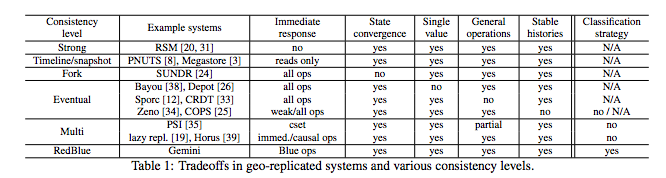
\includegraphics[width=10cm]{pic1.jpg}
\centering
\end{figure}
\end{frame}

% --------------------------------------------------- Slide --5

\begin{frame}
\frametitle{Related Work: Levels of Consistency}
\begin{enumerate}
\item Strong Consistency - Replicated systems behave like a single server that serialize all operations.
\item Timeline/Snapshot Consistency - There is a total order for updates to the service state but gives the option of reading a consistent but dated view of the service.
\item Fork Consistency - Relaxes strong consistency by allowing users to observe distinct causal histories.
\item Eventual Consistency - All replicas "eventually" diverge at some state.
\item Multi Consistency - Other systems expose multiple values from divergent branches in operation replies either directly to the client or to an application-specific conflict resolution procedure.
\item RedBlue Consistency - Operations have multiple consistency levels
\end{enumerate}

\end{frame}


% --------------------------------------------------- Slide --6

\begin{frame}
\frametitle{Related Work: Other}
\begin{enumerate}
\item Consistency Rationing - Consistency guarantees associated with the data instead of the operation. Also switches consistency levels at runtime.
\item TACT - bounds the amount of inconsisteny based on parameters like numeric errors, order errors, staleness, etc.
\end{enumerate}

\end{frame}


% --------------------------------------------------- Slide --7

\begin{frame}
\frametitle{System Model - Assumptions}
\begin{enumerate}
\item A distributed system with state fully replicated across $k$ sites denoted $site_0 \ldots site_{k-1}$
\item $s \in S$ denotes a system state and $u,v \in O$ a set of operations. 
\item Initial State - $S_0$. When operation $u$ is applied it goes to state $S'$. So $S' = S + u$
\item $ \forall$ S $\in S,$ S$+u+v = $ S $+v+u$
\item A state $S$ is valid if it satisfies all these invariants.
\item Each $u$ is submitted to one site which is called $u's$ primary site and denoted by $site(u)$.
\item The system later replicates $u$ to the other sites.
\end{enumerate}

\end{frame}

% --------------------------------------------------- Slide --8

\begin{frame}
\frametitle{RedBlue Consistency}
\begin{itemize}
\item RedBlue order $\colon$ Given a set of operations $U = B \cup R$,where $B \cap R = \emptyset$, a RedBlue order is a partial order $O = ( U, \prec)$ with the restriction that $\forall u,v \in R$ such that $u \neq v, u \prec v $ or $v \prec u$ ($i.e.$ red operations are totally ordered).

\item Causal Serialization $\colon$ Given a site $i$, $O_i = (U, <)$ is an $i$-causal serialization(or short, a causal serialization) of RedBlue order $O = ( U, \prec)$ if 
 \begin{enumerate}
\item$O_i$ is a linear extension of O ($i.e$, < is a total order compatible with the partial order $\prec$ ) 
\item for any two operations $u,v \in U$, if $site(v) = i$ and $u < v$ in $O_i$ then $u \prec v$
\end{enumerate} 
\end{itemize}

\end{frame}


% --------------------------------------------------- Slide --8

\begin{frame}
\frametitle{RedBlue Consistency - Definition}
\begin{itemize}
\item RedBlue consistency $\colon$ A replicated sytem is O-RedBlue consistent(or short, RedBlue consistent) if each site i applies operations according to an i-causal serialization of RedBlue order $O$.
\end{itemize}
\end{frame}

% --------------------------------------------------- Slide --8-1

\begin{frame}
\frametitle{Example}
\begin{figure}[t]
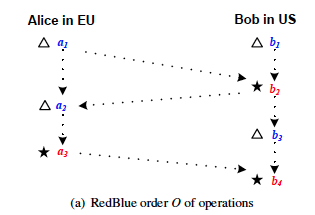
\includegraphics[width=10cm]{pic2.jpg}
\centering
\end{figure}
\end{frame}

% --------------------------------------------------- Slide --8-2

\begin{frame}
\frametitle{Example}
\begin{figure}[t]
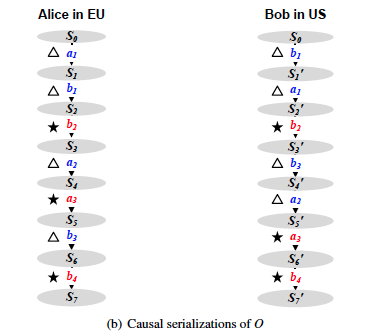
\includegraphics[width=7cm]{pic3.jpg}
\centering
\end{figure}
\end{frame}

% --------------------------------------------------- Slide --9

\begin{frame}
\frametitle{State Convergence }
\begin{itemize}
\item A RedBlue consistent system is state convergent if all causal serializations of the underlying RedBlue order $O$ reach the same state $S$.
\end{itemize}

\end{frame}

% --------------------------------------------------- Slide --9-1

\begin{frame}
\frametitle{State Convergence:Example }
\begin{figure}[t]
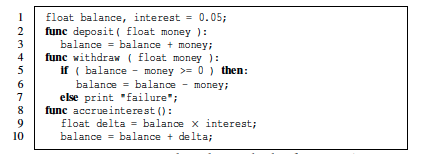
\includegraphics[width=10cm]{pic4.jpg}
\centering
\end{figure}

\end{frame}

% --------------------------------------------------- Slide --9-2

\begin{frame}
\frametitle{State Convergence:Example }
\begin{figure}[t]
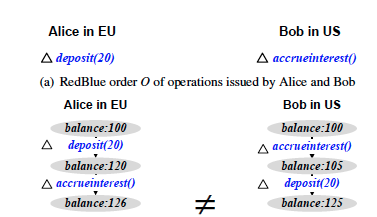
\includegraphics[width=10cm]{pic5.jpg}
\centering
\end{figure}
\end{frame}


% --------------------------------------------------- Slide --9-3

\begin{frame}
\frametitle{State Convergence:Theorem }
\begin{theorem}
Given a RedBlue order O, if all blue operations are globally commutative then any $O$-RedBlue consistent system is state convergent
\end{theorem}

\end{frame}


% --------------------------------------------------- Slide --10

\begin{frame}
\frametitle{Replicating side effects -Generator Operation and Shadow Operation}
\begin{enumerate}
\item Generator Operation $g_u$ - executed only at primary site against some system state $S$.
\item Shadow Operation $h_u(S)$ - executed at every site(including the primary site)
\end{enumerate}
\end{frame}


% --------------------------------------------------- Slide --10--1

\begin{frame}
\frametitle{Replicating side effects - Defining shadow operations}
\begin{enumerate}
\item Correct Generator/ Shadow Operations $\colon$ The decomposition of operation $u$ into generator and shadow operations is correct if for all states $S$, the generator operation $g_u$ has no effect and the generated shadow operation $h_u(S)$ has the same effect as $u$, $i.e.$, for any state $S: S + g_u = S$ and $S + h_u(S) = S + u$
\end{enumerate}

\end{frame}

% --------------------------------------------------- Slide --11

\begin{frame}
\frametitle{Replicating side effects -Revisiting RedBlue consistency}
\begin{enumerate}
\item Given a site $i$, $O_i = (U \cup V_i, <)$ is an $i$-causal serialization of RedBlue order $O = (U , \prec)$ if
\begin{itemize}
\item $O_i$ is a total order;
\item $(U,<)$ is a linear extension of $O$;
\item For any $h_v(S) \in U$ generated by $g_v \in V_i$, $S$ is the state obtained after applying the sequence of shadow operations preceeding $g_v$ in $O_i$;
\item For any $g_v \in V_i$ and $h_u(S) \in U$, $h_u(S) < g_v$ in $O_i$ iff $h_u(S) \prec h_v(S')$ in $O$.
\end{itemize}

\end{enumerate}

\end{frame}


% --------------------------------------------------- Slide --11-1

\begin{frame}
\frametitle{Shadow Banking and Invariants - Example}
\begin{figure}[t]
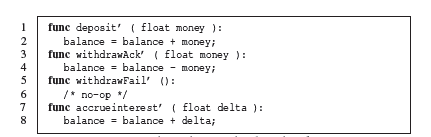
\includegraphics[width=10cm]{pic6.jpg}
\centering
\end{figure}

\end{frame}

% --------------------------------------------------- Slide --11-2

\begin{frame}
\frametitle{Shadow Banking and Invariants - Example}
\begin{figure}[t]
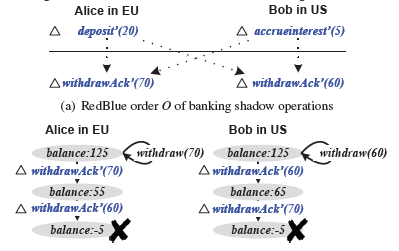
\includegraphics[width=10cm]{pic7.jpg}
\centering
\end{figure}

\end{frame}

% --------------------------------------------------- Slide --11-3

\begin{frame}
\frametitle{Shadow Banking and Invariants - Example}
\begin{itemize}
\item Invariant Safe - Shadow operation $h_u(S)$ is invariant safe if for all valid states $S$ and $S'$, the state $S' + h_u(S)$ is also valid.
\end{itemize}
\begin{theorem}
If all shadow operations are correct and all blue shadow operations are invariant safe and globally commutative,then for any execution of that system that is RedBlue consistent, no site is ever in an invalid state.
\end{theorem}
\end{frame}

% --------------------------------------------------- Slide --12

\begin{frame}
\frametitle{What can be blue? What can be red?}
The procedure for deciding which shadow operations can be blue or must be red if a RedBlue consistent system is to provide both state convergence and invariant preservation:
\begin{enumerate}
\item For any pair of non-commutative shadow operations $u$ and $v$, label both $u$ and $v$ red.
\item For any shadow operation $u$ that may result in an invariant being violated, label $u$ red.
\item Label all non-red shadow operations blue.
\end{enumerate}

\end{frame}

% --------------------------------------------------- Slide --12-1

\begin{frame}
\frametitle{Shadow Banking and Invariants - Example}
\begin{figure}[t]
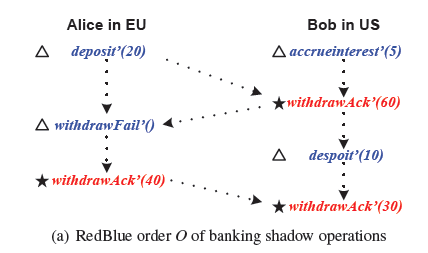
\includegraphics[width=10cm]{pic8.jpg}
\centering
\end{figure}

\end{frame}

% --------------------------------------------------- Slide --12-2

\begin{frame}
\frametitle{Shadow Banking and Invariants - Example}
\begin{figure}[t]
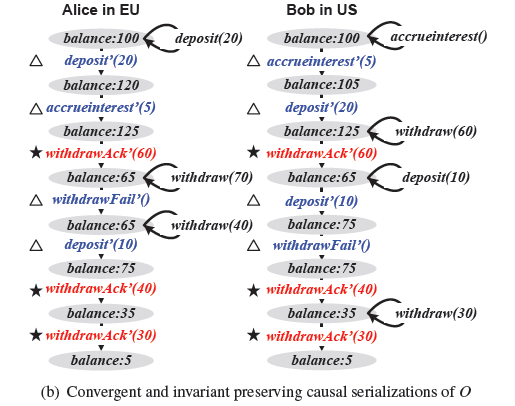
\includegraphics[width=9cm]{pic9.jpg}
\centering
\end{figure}

\end{frame}




% --------------------------------------------------- Slide --14

\begin{frame}
\frametitle{Gemini Design and Implementation - Prototype}
\begin{enumerate}
\item It consisted of 10K lines of java code and uses MySQL as its storage back-end
\item Each Gemini site consists of :
\begin{itemize}
\item a storage engine
\item a proxy server
\item a concurrency coordinator
\item a data writer
\end{itemize}
\item The single site is replicated across multiple sites.
\end{enumerate}
\end{frame}

% --------------------------------------------------- Slide --14-1

\begin{frame}
\frametitle{Gemini Design and Implementation - Basic Flow}
\begin{enumerate}
\item User issues request to a proxy server located at the closest site.
\item The proxy server processes the request by executing an appropriate application transaction which is implemented as a single Gemini operation. 
\item Storage Engine - Relational Database
\item Scratchpad Operations - Temporary tables
\end{enumerate}
\end{frame}

% --------------------------------------------------- Slide --14-1

\begin{frame}
\frametitle{Gemini Design and Implementation - Basic Flow}
\begin{enumerate}
\item User issues request to a proxy server located at the closest site.
\item The proxy server processes the request by executing an appropriate application transaction which is implemented as a single Gemini operation. 
\item Storage Engine - Relational Database
\item Scratchpad Operations - Temporary tables
\end{enumerate}
\end{frame}





% --------------------------------------------------- Slide --14-2

\begin{frame}
\frametitle{Gemini Design and Implementation - Failure Handling}
\begin{enumerate}
\item Isolated Component Failure - Standard state machine replication techniques can be employes to make each component robust.
\item Site Failure - A fault tolerance consensus protocol like Paxos can be used.
\item Operation Propagation - This can be addressed by using standard techniques for exchaning causal logs or reliable multicast.
\item Cross-session monotonicity - This can be addressed by allowing the user to specify a "last read" version when starting a new session or requiring the user to cache all relevant requests in order to reply them when connecting to a new site.
\end{enumerate}
\end{frame}

% --------------------------------------------------- Slide --15

\begin{frame}
\frametitle{Case Studies}
\begin{itemize}
\item TPC-W shopping cart benchmark
\item RUBiS auction benchmark
\item Quoddy social networking application
\end{itemize} 
Two main tasks :
\begin{itemize}
\item Decomposing the application into a generator and shadow operation
\item Labeling the shadow operations appropriately
\end{itemize}
\end{frame}

% --------------------------------------------------- Slide --15-1

\begin{frame}
\frametitle{Original application to RedBlue Consistent}
\begin{figure}[t]
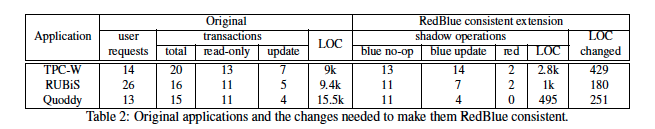
\includegraphics[width=9cm]{pic10.jpg}
\centering
\end{figure}

\end{frame}


% --------------------------------------------------- Slide --15-2

\begin{frame}
\frametitle{TPC-W}
\begin{itemize}
\item Serves 14 different user requests such as browsing, searching, adding products to a shopping cart or placing an order.
\item Each user request generates one to four transactions that access state stored across eight different tables.
\item Shopping cart can be shared by multiple users across multiple sessions.
\end{itemize}
\end{frame}

% --------------------------------------------------- Slide --15-3

\begin{frame}
\frametitle{TPC-W - Writing TPC-W generator and shadow operations}
\begin{figure}[t]
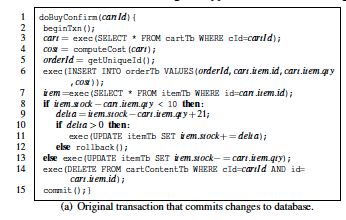
\includegraphics[width=10cm]{pic11.jpg}
\centering
\end{figure}
\end{frame}

% --------------------------------------------------- Slide --15-4

\begin{frame}
\frametitle{TPC-W - Writing TPC-W generator and shadow operations}
\begin{figure}[t]
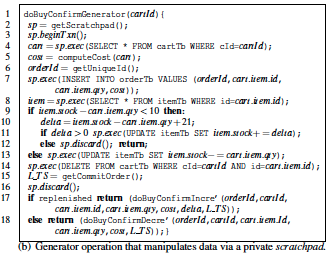
\includegraphics[width=10cm]{pic12.jpg}
\centering
\end{figure}
\end{frame}

% --------------------------------------------------- Slide --15-5

\begin{frame}
\frametitle{TPC-W - Writing TPC-W generator and shadow operations}
\begin{figure}[t]
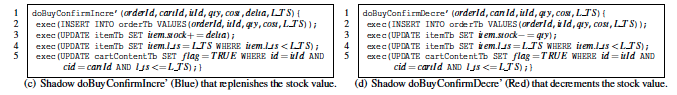
\includegraphics[width=10cm]{pic13.jpg}
\centering
\end{figure}
\end{frame}


% --------------------------------------------------- Slide --16

\begin{frame}
\frametitle{Evaluation-Experimental Setup}
\begin{itemize}
\item Experiments were run on Amazon EC2 using 5 virtual machine instances located in 5 sites - US east(UE), US west(UW), Ireland(IE), Brazil(BR) and Singapore(SG).
\item Each VM has 8 virtual cores and 15 GB of RAM. VMs run Debian 6( Squeeze) 64 bit, MYSQL 5.5.18,Tomcat 6.0.35 and Sun Java SDK 1.6.
\end{itemize}
\end{frame}


% --------------------------------------------------- Slide --16-1

\begin{frame}
\frametitle{Evaluation-Experimental Setup}
\begin{figure}[t]
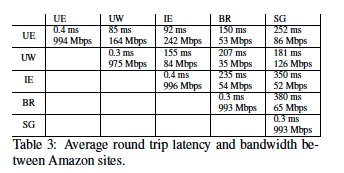
\includegraphics[width=10cm]{pic14.jpg}
\centering
\end{figure}
\end{frame}


% --------------------------------------------------- Slide --17

\begin{frame}
\frametitle{Evaluation-Microbenchmark}
\begin{itemize}
\item Each user issues requests accessing a random record from a MySQL database.
\item Each request maps to a single shadow operation
\item A request is blue if it maps to a blue shadow operation and red otherwise
\item Dataset consists of 10 tables,each initialized with 1,000,000 records, each record has 1 text and 4 integer attributes. The total size of the dataset is 1.0 GB.
\end{itemize}
\end{frame}


% --------------------------------------------------- Slide --17-1

\begin{frame}
\frametitle{Evaluation-Microbenchmark}
\begin{figure}[t]
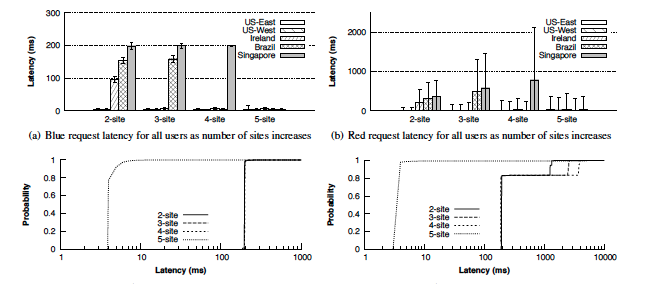
\includegraphics[width=10cm]{pic15.jpg}
\centering
\end{figure}
\end{frame}


% --------------------------------------------------- Slide --18

\begin{frame}
\frametitle{Evaluation-Peak Throughput}
\begin{figure}[t]
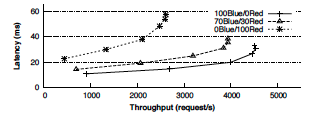
\includegraphics[width=10cm]{pic16.jpg}
\centering
\end{figure}
\end{frame}

% --------------------------------------------------- Slide --19

\begin{frame}
\frametitle{Evaluation-TPC-W}
\begin{figure}[t]
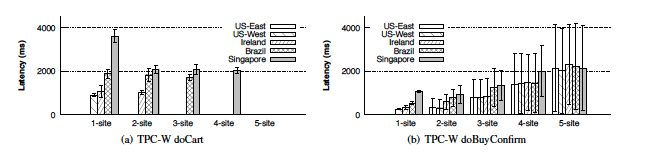
\includegraphics[width=5cm]{pic17.jpg}
\centering
\end{figure}
\begin{figure}[t]
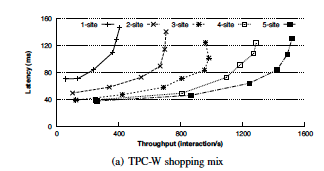
\includegraphics[width=5cm]{pic18.jpg}
\centering
\end{figure}
\end{frame}



% --------------------------------------------------- Slide --20

\begin{frame}
\frametitle{Conclusion}

\end{frame}
% --------------------------------------------------- Slide --19-1

\begin{frame}
\frametitle{Evaluation-TPC-W}
\begin{figure}[t]
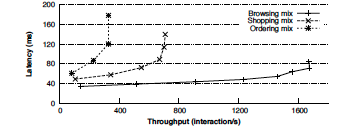
\includegraphics[width=5cm]{pic19.jpg}
\centering
\end{figure}
\begin{figure}[t]
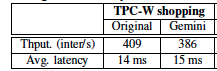
\includegraphics[width=5cm]{pic20.jpg}
\centering
\end{figure}
\end{frame}




%%% BEGIN SHANNON SECTION %%%
% --------------------------------------------------- Slide --

\section{Lloyd et al.} 

\begin{frame}
\frametitle{Paper 2: Lloyd et al.}

\textbf{Stronger Semantics for Low-Latency Geo-Replicated Storage} \newline
\textit{Proceedings of the 10th USENIX Symposium on Networked Systems Design and Implementation (NSDI’13)} \newline
Wyatt Lloyd, Michael J. Freedman, Michael Kaminsky, and David G. Andersen \newline
April 2013 \newline

\end{frame}

% --------------------------------------------------- Slide --
\begin{frame}
\frametitle{Motivation}
\begin{itemize}

\item Consider an example from Facebook
\pause\item Joe performs 2 actions:
	\begin{itemize}
		\item Defriend boss.
		\item Make snarky comment about boss and promise to quit.
	\end{itemize}
\item In an \textcolor{red}{eventually} consistent system, these can be viewed in the wrong order for a period time, earning Joe his first unemployment check.
\item This won't happen with \textcolor{green}{causal} consistency.

\end{itemize}  
\end{frame}

% --------------------------------------------------- Slide --
\begin{frame}
\frametitle{Consistency - Causal versus Eventual}
\begin{itemize}
	\item Eventual Consistency
	\begin{itemize}
		\item At some point, the replicas will converge
		\item Until then, no guarantees
		\item \textcolor{red}{Joe's boss might see his whining.}	
	\end{itemize}

\pause \item Causal Consistency
	\begin{itemize}
		\item At a single processor, serial order of events determines causal order
		\item Reads are causally ordered after their writes across processors
		\item Transitive closure of these two properties
		\item \textcolor{green}{Joe is safe to gripe.}
	\end{itemize}

\end{itemize}  
\end{frame}


% --------------------------------------------------- Slide --
\begin{frame}
\frametitle{Overview}
\begin{itemize}

\item We modify an eventually consistent system to get a causally consistent one
\item Extend Cassandra to get Eiger
\item Take slight hit in \textcolor{red}{throughput} \newline to get stronger version of \textcolor{green}{consistency}
\item Maintain low latency

\end{itemize}  
\end{frame}

% --------------------------------------------------- Slide --
\begin{frame}
\frametitle{Contributions of the paper} 
\begin{itemize}
\item Eiger
	\begin{itemize}
		\item Low Latency
		\item High throughput (slightly lower than Cassandra)
		\item Causal Consistency (rather than eventual as in Cassandra)
	\end{itemize}
\item Read Only Algorithm
\item Write Only Algorithm
\end{itemize}  
\end{frame}

% --------------------------------------------------- Slide --
\begin{frame}
\frametitle{Background}
\begin{itemize}
\item Cassandra
	\begin{itemize}
		\item Designed by Facebook to search inbox messages (has since been replaced by Hbase for better scalability)
		\item Other companies are still using Cassandra (e.g., Netflix and Apple)
		\item Allows Eventual or Strong Consistency
		\item If you want low latency, Eventual is the only option
	\end{itemize}
%\pause \item COPS
\end{itemize}  
\end{frame}





% --------------------------------------------------- Slide --
\begin{frame}
\frametitle{Eiger: Column Family Data Model}
\begin{itemize}
\item Hierarchical Column families: 3 tiers

\item Example:
	\begin{itemize}
		\item Super Family = Association
		\item Family = Friends
		\item Column = Alice
	\end{itemize}
\end{itemize}  
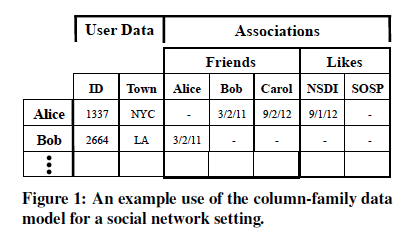
\includegraphics[scale=0.5]{Figure_Lloyd_ColumnHierarchy.png}
\end{frame}


% --------------------------------------------------- Slide --
\begin{frame}
\frametitle{Eiger: Operations}
\begin{itemize}
\item Cassandra has only 3 operations (key determines row)
	\begin{itemize}
		\item Insert(table, key, rowMutation)
		\item Get(table, key, columnName)
		\item Delete(table, key, columnName)
	\end{itemize}
\pause \item Eiger adds more complex transactions
	\begin{itemize}
		\item Batch Mutate: insert or delete multiple keys as a group of independent operations
		\item Atomic Mutate: insert or delete multiple keys in a single atomic batch
		\item Multiget Slice: read multiple columns/keys
		\item Multiget Slice by Time
	\end{itemize}	
\end{itemize}  
\end{frame}

% --------------------------------------------------- Slide --
\begin{frame}
\frametitle{Eiger: Client Library}
\begin{itemize}
\item Manages read and write algorithms
\item Tracks causality by maintaining 1-hop dependencies
\item For an atomic write, no write is applied in a cluster until after all the dependencies have been applied.  \textcolor{red}{This is necessary for causal consistency.}
\item Dependencies are on operations rather than values (as in COPS). 
\end{itemize}  
\end{frame}

% --------------------------------------------------- Slide --
\begin{frame}
\frametitle{Eiger: One-Hop Dependencies}

Example:  For w8, only w6 and w5 are stored.

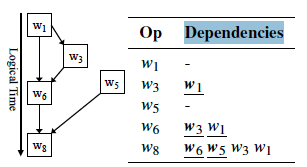
\includegraphics[scale=0.5]{Figure_Dependencies.png}
\end{frame}

% --------------------------------------------------- Slide --
\begin{frame}
\frametitle{Eiger: Read Algorithm}
\begin{itemize}
\item Non-blocking: other processes can read
\item Partition Tolerant
\item 1 or 2 rounds of non-blocking parallel reads
\end{itemize}  
\end{frame}

% --------------------------------------------------- Slide --
\begin{frame}
\frametitle{Eiger: Read Algorithm}
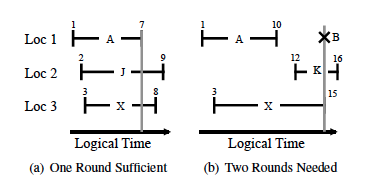
\includegraphics[scale=0.80]{Figure_Read.png}
\end{frame}

% --------------------------------------------------- Slide --
\begin{frame}
\frametitle{Eiger: Read Algorithm}
\begin{itemize}
\item Step 1: Find latest lower bound, L
\item Step 2: Find lowest upper bound that is higher than L
\newline If all upper bounds are higher than L then we are done.  If not, continue. 
\item Step 3: For any reads that had an upper bound lower than L, read again.
\end{itemize}  
\end{frame}


% --------------------------------------------------- Slide --
\begin{frame}
\frametitle{Eiger: Write Algorithm}
\begin{itemize}
\item Atomically write set of keys
\item Lock free (and thus low latency)
\item Does not block concurrent reads
\end{itemize}  
\end{frame}



% --------------------------------------------------- Slide --
\begin{frame}
\frametitle{Eiger: Write Algorithm}
Three parties involved
\begin{itemize}
	\item Client - requests write to many servers
	\item Coordinator server - a randomly chosen server from list of transaction destinations
	\item Cohort server - all other destinations
\end{itemize}  
\end{frame}



% --------------------------------------------------- Slide --
\begin{frame}
\frametitle{Eiger: Write Algorithm}
Three parties involved
\begin{itemize}
	\item Step 1: Break up transaction into a separate request for each destination.
	\item Step 2: Randomly choose coordinator and send transactions to all destinations.
	\item Step 3: Cohort servers send notification to coordinator.
	\item Step 4: Coordinator runs dependency checks
	\item Step 5: 2 Phase commit (to ensure all-or-nothing)
	\item Step 6: Coordinator sends ACK to client
\end{itemize}  
\end{frame}

% --------------------------------------------------- Slide --
\begin{frame}
\frametitle{Eiger: Write Algorithm}
Example:
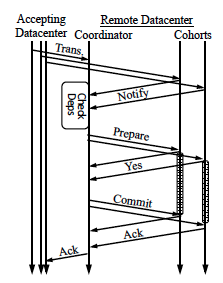
\includegraphics[scale=0.5]{Figure_Write_Transaction.png}
\end{frame}

% --------------------------------------------------- Slide --
\begin{frame}
\frametitle{Evaluation}
Comparison to Cassandra:
\begin{itemize}
	\item Within 7\% of throughput Using Facebook data
\end{itemize}
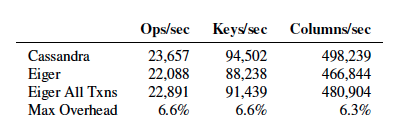
\includegraphics[scale=0.6]{Figure_Facebook_Throughput.png}  
\end{frame}

% --------------------------------------------------- Slide --
\begin{frame}
\frametitle{Evaluation}
Comparison to Cassandra:
\begin{itemize}
	\item Cassandra had median latency of 0.38ms, whereas Eiger had 0.78ms
	\item Thus, there is about a factor of 2 difference
	\item Strongly Consistent Cassandra had 85.21ms latency
\end{itemize}
\end{frame}


% --------------------------------------------------- Slide --
\begin{frame}
\frametitle{Evaluation}
Almost linear scaling:
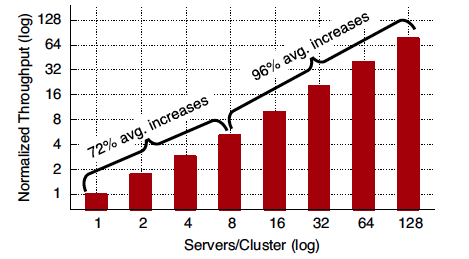
\includegraphics[scale=0.6]{Figure_Almost_Linear.png}  
\end{frame}







% --------------------------------------------------- Slide --
\begin{frame}
\frametitle{Conclusion: Relationship between 2 Papers}
\begin{itemize}
\item Similarities
	\begin{itemize}
		\item Geo-replicated Systems
		\item Provide improvement in consistency
	\end{itemize}
\item Differences
	\begin{itemize}
		\item Li: Latency versus Consistency.
			\begin{itemize}
				\item Separate operations into those that must be consistent and those that need not.
			\end{itemize}
		\item Lloyd: Consistency versus Throughput (requiring low latency)
			\begin{itemize}
				\item Extend previous system to offer causal consistency with small hit to throughput.
			\end{itemize}
	\end{itemize}

\end{itemize}  
\end{frame}

% --------------------------------------------------- Slide --
\begin{frame}
\frametitle{The End}
\LARGE{Thank you!}
\end{frame}


% --------------------------------------------------- Slide --

\section{Bibliography} 

\begin{frame}
\frametitle{Bibliography}


%%% SHANNON'S REFERENCES
\begin{itemize}
\item \textbf{Stronger Semantics for Low-Latency Geo-Replicated Storage}, 
\textit{Proceedings of the 10th USENIX Symposium on Networked Systems Design and Implementation (NSDI’13)}, 
Wyatt Lloyd, Michael J. Freedman, Michael Kaminsky, and David G. Andersen, 
April 2013

\item \textbf{Out in the Open: The Abandoned Facebook Tech That Now Helps Power Apple}, 
\textit{www.wired.com}
, Klint Finley, Aug. 4, 2014

\item \textbf{A Short Primer on Causal Consistency}, 
\textit{;login: The Usenix Magazine Volume 38, Number 4}, 
Wyatt Lloyd, Michael J. Freedman, Michael Kaminsky, and David G. Andersen, , August 2013

\item \textbf{Netflix's Viewing Data: How We Know Where You Are in House of Cards},
\textit{http://techblog.netflix.com/search/label/Cassandra}
January 27, 2015

%\item \textit{http://wiki.apache.org/cassandra}

\end{itemize}  
\end{frame}


\end{document} 